\documentclass[a4paper,10pt,hidelinks]{article}

\usepackage{tikz}
\usepackage{hyperref}
\usepackage{algorithm}
\usepackage{algpseudocode}

\usepackage{listings}
\lstset{
    numbers=left,
    breaklines=true
}

\newcommand{\algorithmautorefname}{Algorithm}

%opening
\title{Practical Assignment 2\\
Social Network Analysis}
\author{Bert Peters\\
s1147919}

\begin{document}

\maketitle

\section{Clustering Coefficient}

\begin{enumerate}
 \item A tree, by definition, has no loops, and therefore has a clustering coefficient of 0. Another example is a bipartite graph. This type of graph can only have cycles of at least length 4. This is because it is impossible for two edges in the same partition to have a connection. Cycles of length 4 do not contribute to the clustering coefficient, because that only counts the number of triangles, i.e. the number of cycles of length 3.

 \item There are several possible such graphs. One of them is shown in \autoref{fig:graph-no-clustering}.
 
 \item Contructing an unclustered graph is trivial for when $m \leq n$, because we can construct a circle graph of size $n$ and remove edges to arrive at the desired number of edges. The algorithm is shown in \autoref{algo:algo-no-clustering}.
\end{enumerate}

\begin{figure}
    \centering
    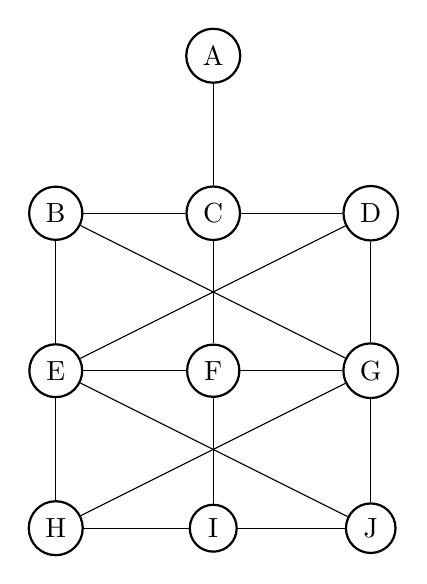
\begin{tikzpicture}[every node/.style={draw=black,thick,circle}]
        \node (A) at (0,4){A};
        \node (B) at (-2,2){B};
        \node (C) at (0,2){C};
        \node (D) at (2,2){D};
        \node (E) at (-2,0){E};
        \node (F) at (0,0){F};
        \node (G) at (2,0){G};
        \node (H) at (-2,-2){H};
        \node (I) at (0,-2){I};
        \node (J) at (2,-2){J};
        
        \draw (A) -- (C);
        \draw (B) -- (C);
        \draw (C) -- (D);
        \draw (B) -- (E);
        \draw (C) -- (F);
        \draw (E) -- (F);
        \draw (D) -- (G);
        \draw (F) -- (G);
        \draw (E) -- (H);
        \draw (H) -- (I);
        \draw (F) -- (I);
        \draw (I) -- (J);
        \draw (G) -- (J);
        
        \draw (B) -- (G);
        \draw (D) -- (E);
        
        \draw (E) -- (J);
        \draw (G) -- (H);

    \end{tikzpicture}
    \caption{An undirected graph with 10 nodes, 15 edges, and a clustering coefficient of 0.}
    \label{fig:graph-no-clustering}
\end{figure}

\begin{algorithm}
\caption{Constructing a graph with no clustering.}
\label{algo:algo-no-clustering}

\begin{algorithmic}
    \State $E \gets \emptyset$
    \Comment{TODO}
\end{algorithmic}

\end{algorithm}

\section{Densest Subgraph}

We start by computing the average degree and the current density. For a graph with a given $n, m$ this is easy, because the average degree is $\frac{2m}{n}$ and the density is half of that. We run our algortihm, by iteratively removing the nodes with a degree lower than the average degree from our $V$ and $E$, and repeat the process until we cannot delete nodes anymore.

Using the above algorithm, we arrive at the results as shown in \autoref{tab:densest-subgraph}. We see that after iteration 1, we already find our maximum, with a density of 1.5. After that, we still delete nodes twice, until we arrive at a graph with two nodes and cannot delete nodes anymore.

\begin{table}
    \centering
    \begin{tabular}{r || l | r | r}
        Iteration & Subgraph & Density & Avg. degree\\
        \hline
        0   & $\{A B C D E F H I J K L\}$ & $\frac{16}{11} \approx 1.45 $ & $\frac{32}{11} \approx 2.9 $ \\
        1   & $\{A B E F J K\}$ & $ \frac{9}{6} = 1.5 $ & $ \frac{18}{6} = 3 $ \\
        2   & $\{B E F J\}$ & $\frac{5}{4} = 1.25$ & $\frac{10}{4} = 2.5$ \\
        3   & $\{E F\}$ & $\frac{1}{2} = 0.5$ & $\frac{2}{2} = 1$
    \end{tabular}
    \caption{Using the greedy algorithm to find the densest subgraph.}
    \label{tab:densest-subgraph}
\end{table}

\section{Twitter Network Extraction}

\subsection{Parsing the tweets}

We parse the tweets using a python script in \autoref{lst:preprocess}. It takes a list of files as arguments from the command line or data from the standard input. It attempts to parse out a mention using a regular expression. The expression used is a non-word character, followed by an '@', followed by at most 15 word characters, followed by by a non-word character.

\lstinputlisting[language=python,label=lst:preprocess,caption=Preprocessing script for the twitter data.,float]{preprocess.py}

\end{document}
